\subsection{Q3: Exploration 3.4.2 (Page 87)}
\label{Q3:Expl 3.4.2 SubSection}

\subsubsection{Task 3.7}
\label{Q1:Expl 3.4.2 (3.7) SubSubSection}

\begin{tcolorbox}[colback=gray!20!white,colframe=gray!20!white]
  \emph{\textbf{Question 3.7 (a)} Given the pattern of weights, what is the minimal number of units that need to be clamped to produce pattern completion to the full 8? You can determine your answer by toggling off the units in the event pattern one-by-one until the network no longer produces the complete pattern when it is Run (don’t forget to press Apply in the environment window after clicking).\textbf{(b)} The $g_{bar\_l}$ parameter can be altered to lower this minimal number. What value of this parameter allows completion with only one input active? [Mark: 6]} 
\end{tcolorbox} 
\vspace{0.5cm}

With 17 units turned on, the pattern is a visible whereas when 18 units are active the the number 8 is not display at full, this is because due to only 17 units being connected to the receiving unit. $g_{bar\_l}$ can be changed from a value of 7 to 3 to which only one input is active.

\begin{figure}[H]
\centering
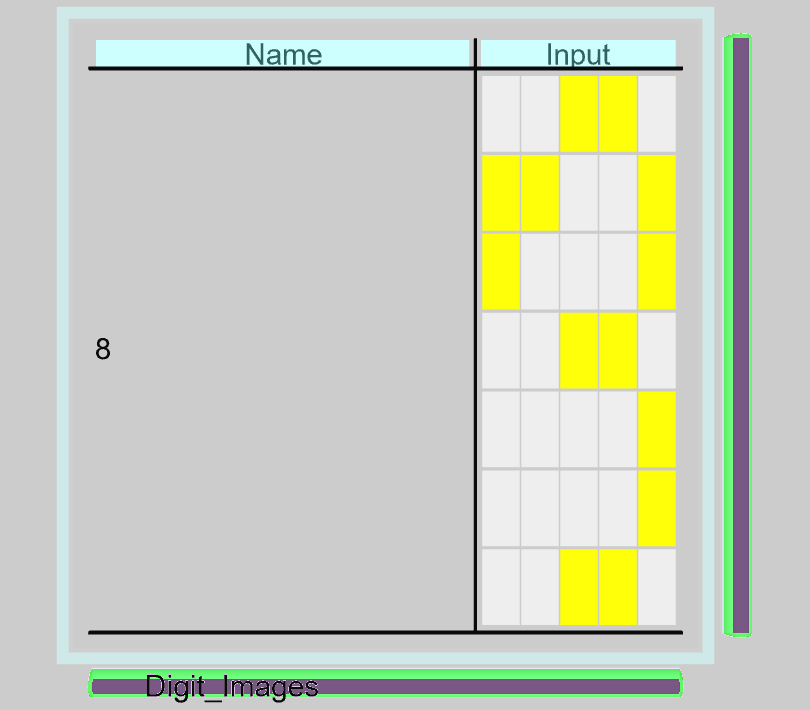
\includegraphics[scale=0.5]{Media/Main/EQ3/S0.png}
\caption{.}
\label{Q3.2}
\end{figure}

\subsubsection{Task 3.8}
\label{Q1:Expl 3.4.2 (3.8) SubSubSection}

\begin{tcolorbox}[colback=gray!20!white,colframe=gray!20!white]
  \emph{\textbf{Question 3.8 (a)} What happens if you activate only inputs which are not part of the 8 pattern? Why? \textbf{(b)} Could the weights in this layer be configured to support the representation of another pattern in addition to the 8 (such that this new pattern could be distinctly activated by a partial input), and do you think it would make a difference how similar this new pattern was to the 8 pattern? Explain your answer. [Mark: 7]} 
\end{tcolorbox} 
\vspace{0.5cm}

When inputs are activated that aren't part of the number 8 digits pattern the image disappears because the weight values of the unit is equal 0. The new pattern could be the number 3 digits as shown in \cref{Q3.2} as enough input units are activated to produce the number 3 digit pattern as it uses the same pattern units as the number 8 digit minus a few units.